\section{Algorithms}
In recent years, methods of meta learning have emerged one after another. Previous% [77], [78]
categorizations of meta-learning methods tend to produce a three-way taxonomy across optimization-based methods, model-based (or black box) methods, and metric-based (or non-parametric) methods.
Today we mainly introduce the most famous example of optimization-based methods, MAML, which is to learn a good initialization for the parameters, and then use a small amount of updates to train new tasks on the basis of this initialization.

\subsection{MAML}
According to the above introduction, we can realize that: From a macro perspective, meta learning uses tasks as ``samples" for learning! So in general, we will divide the data into $Meta\_train$ and $Meta\_test$, where $Meta\_train$ contains data from multiple tasks, and can be divided into $D\_train$ and $D\_test$, which are used for training and testing respectively.

Since current machine learning methods all perform gradient updates, and the focus of MAML is on gradient updates, it can also be regarded as a gradient-based meta learning method.

The core idea of MAML is actually very simple. In each iteration step, there will be an initial parameter $\theta$, which is used to update the gradient of $K$ tasks in $D\_train$ and achieve new $\theta'_i$ of different tasks. After all $\theta'_i$ optimized on $D\_train$, we update the global parameter $\theta$ on K tasks in $D\_test$(see Figure~\ref{fig:graph}).

\begin{figure}[h]
  \centering
  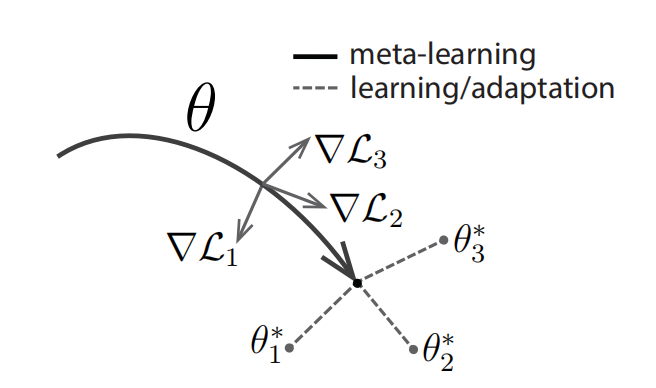
\includegraphics[totalheight=1.5in]{fig1.png}
  \caption{Diagram of our model-agnostic meta-learning algorithm (MAML)} \label{fig:graph}
\end{figure}

The gray branch lines in the figure represent the update direction of $\theta$ on different tasks, and the black line represents the final optimization of the model parameters, which can prevent the parameters from overfitting on a certain task. The last dotted lines represent processes of adaptation to new tasks, which is referred to as the fine-tune of the model parameters.

The gradient-based solution is adaptive to different kinds of learning tasks. Algorithm \ref{MAML} is the generalization of this model.



\begin{algorithm}[h]
  \caption{Model-Agnostic Meta-Learning}
  \label{MAML}
  \begin{algorithmic}[1]
    \REQUIRE $p(\mathcal{T})$: distribution over tasks
    \REQUIRE $\alpha, \beta$: step size hyperparameters
    \STATE randomly initialize $\theta$
    \WHILE {not done}
    \STATE Sample batch of tasks $\mathcal{T}_i \sim p(\mathcal{T})$
    \FORALL {$\mathcal{T}_i$}
    \STATE Evaluate $\nabla_\theta \mathcal{L}_{\mathcal{T}_i} (f_\theta)$ with respect to $K$ examples
    \STATE Compute adapted parameters with gradient descent: $\theta'_i = \theta - \alpha\nabla_\theta \mathcal{L}_{\mathcal{T}_i} (f_\theta)$
    \ENDFOR
    \STATE Update $\theta \leftarrow \theta - \beta\nabla_\theta \Sigma_{\mathcal{T}_i \sim p(\mathcal{T})}\mathcal{L}_{\mathcal{T}_i} (f_{\theta'_i})$
    \ENDWHILE
  \end{algorithmic}
\end{algorithm}

At first, we sample several tasks randomly into a batch.Using each task in the batch, we update the parameters of the model separately, that is, calculate the gradient of each parameter for the support set in a certain task in the batch. Under the setting of N-way K-shot, there should be NK in the support set. The author writes with respect to K examples in the algorithm, and calculates K samples under each class by default. In fact, there are a total of NK samples involved in the calculation. The loss calculation method here is MSE in regression problems and cross-entropy in classification problems. Step 6, the first update of the gradient. After step 4 to step 7, MAML completes the first gradient update. The next thing we need to do is to calculate the second gradient update through gradient by gradient based on the parameters obtained from the first gradient update. The gradient calculated in the second gradient update is directly applied to the original model through SGD, which is the gradient that our model is really used to update its parameters. In other words, the first gradient update is for the second gradient update, and the second gradient update is for updating the model parameters. Regarding the above process, here is an explanation: assuming the original model is, we copied it and got it. In the above, we did backpropagation and update parameters to get the result of the first gradient update. Then, on, we will calculate the second gradient update. At this time, you need to calculate the gradient on (the calculation method is as described in the next step 8), but the gradient update is not the original model. This is how the double gradient is implemented in the code. Step 8 corresponds to the process of the second gradient update. The loss calculation method here is roughly the same as step 5, but there are two differences. One is that we no longer use the loss of each task to update the gradient, but like the common model training process, calculate the total loss of a batch, and perform random gradient descent SGD on the gradient. The other is the sample involved in the calculation here, which is the query set in the task. In our example, 5-way*15=75 samples. The purpose is to enhance the generalization ability of the model on the task and avoid over-fitting. support set. After step 8 is over, the model ends the training in the batch, starts to return to step 3, and continues to sample the next batch.
% \begin{algorithm}
%   \caption{MAML for Few-Shot Supervised Learning}
%   \label{MAML}
%   \begin{algorithmic}[1]
%     \REQUIRE $p(\mathcal{T})$: distribution over tasks
%     \REQUIRE $\alpha, \beta$: step size hyperparameters
%     \STATE randomly initialize $\theta$
%     \WHILE {not done}
%     \STATE Sample batch of tasks $\mathcal{T}_i \sim p(\mathcal{T})$
%     \FORALL {$\mathcal{T}_i$}
%     \STATE Sample $K$ datapoints $\mathcal{D}=\{x^{(j)}, y^{(j)}\}$ from $\mathcal{T}_i$
%     \STATE Evaluate $\nabla_\theta \mathcal{L}_{\mathcal{T}_i} (f_\theta)$ with respect to $K$ examples
%     \STATE Compute adapted parameters with gradient descent: $\theta'_i = \theta - \alpha\nabla_\theta \mathcal{L}_{\mathcal{T}_i} (f_\theta)$
%     \STATE Sample datapoints $D'_i=\{x^{(j)}, y^{(j)}\}$ from $\mathcal{T}_i$ for the meta-update
%     \ENDFOR
%     \STATE Update $\theta \leftarrow \theta - \beta\nabla_\theta \Sigma_{\mathcal{T}_i \sim p(\mathcal{T})}\mathcal{L}_{\mathcal{T}_i} (f_{\theta'_i})$
%     \ENDWHILE
%   \end{algorithmic}
% \end{algorithm}